\documentclass[11pt,letterpaper]{article}
\usepackage{graphicx}
\usepackage{geometry}
\usepackage{amsmath}
\usepackage{hyperref}
\usepackage{url}
\usepackage{natbib}
\usepackage{booktabs}
\usepackage{xcolor}
\usepackage{listings}
\usepackage{microtype}

\geometry{margin=1in}
\hypersetup{colorlinks=true, linkcolor=black, citecolor=black, urlcolor=black}

\title{\textbf{Circular Text Fingerprints: Evaluating ECFP-Inspired Neighborhood\\Hashing for Near-Duplicate Short-Text Detection}}

\author{
  Anonymous Author(s)
}

\date{}

\begin{document}

\maketitle

\begin{abstract}
Detecting near-duplicate text is a fundamental problem in information retrieval, with applications in search consolidation, deduplication, and plagiarism detection. For short texts (8--20 words), traditional $n$-gram shingling produces sparse feature sets, leading to unreliable similarity estimates. We explore Circular Text Fingerprints (CTF), adapting Extended Connectivity Fingerprints (ECFP) from cheminformatics by iteratively hashing each word token together with its neighbors at multiple radii. This approach generates $O(n \cdot R)$ multi-scale features per text, encoding nested token-context patterns. We evaluate CTF on 162,415 test pairs from the Quora Question Pairs benchmark, stratified by text length, comparing against non-degenerate baselines: character 4-gram Jaccard, word-unigram Jaccard, and TF-IDF cosine similarity. Character 4-gram Jaccard achieves the best overall performance at F1=0.6557. CTF ($R=3$) achieves F1=0.6422, performing significantly below the best baseline (McNemar $p{<}0.001$, 95\% CI: $[-0.015,\,-0.012]$). However, stratified analysis reveals that CTF's token-context approach produces stronger recall (90.6\% vs.\ 89.6\%) with lower precision, favoring high-recall applications. We find that iterative neighborhood hashing does not uniformly improve over fixed $n$-gram approaches for short text, but offers interpretable trade-offs: explicit multi-scale token-context encoding at the cost of reduced discrimination. The method remains fully unsupervised and training-free, making it applicable to low-resource and privacy-sensitive settings.
\end{abstract}

\section{Introduction}

\subsection{The Problem}

Near-duplicate detection---identifying text pairs that are substantially similar despite minor variations---is a core task in information retrieval, data cleaning, and content moderation. The problem is particularly acute for short text: question titles (6--15 words), search queries, tweets, and product descriptions. In these cases, the signal-to-noise ratio is inherently low because documents contain fewer distinct features, making reliable similarity estimation challenging.

\subsection{Why It Matters}

The Quora Question Pairs dataset contains over 400,000 question pairs with an average length of 12.8 words. Production systems must process millions of such pairs daily for search consolidation, duplicate detection, and recommendation filtering. An accurate near-duplicate detector with high recall reduces redundant results and improves user experience; a detector with high precision avoids erroneous merges. The trade-off between precision and recall is task-dependent: search consolidation prioritizes recall (find all duplicates), while deduplication prioritizes precision (merge only certain pairs). However, \emph{any} method that performs worse than well-tuned baselines on the same data is unsuitable for deployment, regardless of its theoretical motivation.

\subsection{Why It Is Hard}

Standard near-duplicate detection relies on the Jaccard similarity of $n$-gram shingles: for a 10-word question with 3-gram shingles, only 8 shingles are possible; for a 6-word question, only 4. When Jaccard similarity is estimated from so few features, variance is high and estimates are unreliable. MinHash, the standard baseline, selects the minimum hash value across $k$ independent hash functions applied to $n$-grams, discarding information about which shingles co-occur and in what contexts. This loss of context is particularly damaging for short texts where few $n$-grams are available to begin with.

\subsection{Why Hasn't It Been Solved Before?}

Existing approaches fall into three categories:

\begin{enumerate}
  \item \textbf{Shallow $n$-gram methods} \citep{Broder1997, Broder2000}: MinHash and SimHash are fast and memory-efficient but treat $n$-gram shingles as independent features, losing token-order and context information.

  \item \textbf{Deep learned methods} \citep{Devlin2019, Hu2019}: Neural metric learning and transformer-based models achieve state-of-the-art performance by learning semantic similarity from labeled data. However, they require substantial labeled training data, are computationally expensive at inference time, and are opaque---unsuitable for interpretability-critical or privacy-sensitive settings.

  \item \textbf{Structural methods}: Dependency parsing and tree-edit distance capture grammar but require robust parsers and fail on informal text (queries, social media).
\end{enumerate}

The gap is not in \emph{absolute performance}---neural methods are superior---but in the regime of \textbf{unsupervised, training-free, interpretable methods that work on short text}. Existing unsupervised baselines (character and word $n$-grams) are simple and fast; the question is whether we can improve on them without sacrificing simplicity and interpretability.

\subsection{Our Approach}

We adapt \textbf{Extended Connectivity Fingerprints} (ECFP), a technique from computational chemistry, to text near-duplicate detection. In cheminformatics, ECFP solves an analogous problem: small molecules have few atoms, yet ECFP generates rich multi-scale fingerprints by iteratively hashing each atom's identifier together with its neighbors' current hashes \citep{Rogers2010, Hahn2013}. This produces $O(\text{atoms} \times \text{radius})$ features per molecule---far richer than atom-type counting alone---and is the standard similarity method for molecules in drug discovery \citep{Hahn2013, Maggiora2014}.

We introduce \textbf{Circular Text Fingerprints} (CTF), replacing atoms with word tokens and atomic bonds with token adjacency in sequences. For each text, we: (1) initialize each token with a hash of its surface form; (2) iteratively propagate context by updating each token's feature as $\text{hash}(\text{current\_feature},\,\text{sorted\_neighbors})$; (3) collect all per-token features across all iterations into a set; (4) estimate similarity via exact Jaccard similarity between fingerprint sets.

\subsection{Key Finding and Contributions}

Contrary to the initial hypothesis, CTF does \textbf{not} outperform well-tuned character $n$-gram baselines on the full QQP test set. Character 4-gram Jaccard achieves F1=0.6557 while CTF ($R=3$) achieves F1=0.6422, a statistically significant difference (McNemar $p{<}0.001$). However, this negative result is itself valuable:

\begin{itemize}
  \item \textbf{Methodological contribution}: We identify and fix critical errors in the prior evaluation---a degenerate MinHash baseline ($\tau=0.00$) and insufficient sample size for short-text stratification ($n=9$ pairs)---and provide a replicable methodology with proper statistical testing.

  \item \textbf{Empirical contribution}: We evaluate CTF against multiple non-degenerate baselines (character 4-gram Jaccard, word-unigram Jaccard, TF-IDF cosine) using proper threshold tuning and statistical significance tests (McNemar's test, bootstrap confidence intervals) on a large test set ($n=162{,}415$).

  \item \textbf{Analytical contribution}: We find that CTF trades precision for recall, achieving 90.6\% recall vs.\ 89.6\% for the best baseline---potentially valuable for high-recall applications despite lower F1. Stratified analysis shows CTF underperforms character 4-grams across all text-length strata, contradicting the hypothesis that token-context encoding would dominate on short text.

  \item \textbf{Practical contribution}: CTF remains fully unsupervised, parameter-free after radius selection, and $O(n \cdot R \cdot \text{window})$ complexity, making it deployable in low-resource and privacy-sensitive settings---albeit without performance advantage over simpler baselines.
\end{itemize}

\section{Methods}

\subsection{Circular Text Fingerprints (CTF)}

Given a text sequence tokenized as $T = [t_1, t_2, \ldots, t_n]$, CTF computes a set-valued fingerprint $F_{\text{CTF}}$ as follows:

\textbf{Initialization}: For each token $t_i$, compute an initial feature $h_0(i) = \text{hash}(t_i)$, where $\text{hash}(\cdot)$ is a stable integer hash function (e.g., MurmurHash or SHA-1).

\textbf{Iterative neighborhood propagation}: For $r = 1$ to $R$:
\begin{itemize}
  \item For each token position $i$, define its neighborhood $N(i) = \{j : |i - j| \leq 1,\, j \neq i\}$---the immediate left and right neighbors.
  \item Compute the sorted tuple of neighbor features: $\text{neighbor\_hashes} = \text{sorted}([h_{r-1}(j) \text{ for } j \in N(i)])$.
  \item Update the token's feature: $h_r(i) = \text{hash}((h_{r-1}(i),\, \text{tuple}(\text{neighbor\_hashes})))$.
  \item Add $h_r(i)$ to the feature set: $F_{\text{CTF}} \leftarrow F_{\text{CTF}} \cup \{h_r(i)\}$.
\end{itemize}

\textbf{Fingerprint assembly}: $F_{\text{CTF}} = \{h_0(i) : i \in 1..n\} \cup \{h_r(i) : r \in 1..R,\, i \in 1..n\}$.

The fingerprint size is at most $n \cdot (R+1)$ and grows linearly with text length and radius.

\textbf{Similarity estimation}: For two texts with fingerprints $F_1$ and $F_2$, compute Jaccard similarity:
\[
  J(F_1, F_2) = \frac{|F_1 \cap F_2|}{|F_1 \cup F_2|}
\]
Classify a pair as duplicate if $J \geq \tau$, where $\tau$ is selected on a held-out training set via grid search.

\subsection{Baseline Methods}

\textbf{Character $k$-gram Jaccard} \citep{Broder1997, StanfordIR}: Extract all contiguous $k$-character substrings from each text ($k=4$), compute their set intersection and union, and estimate Jaccard similarity. This is the standard $n$-gram approach in information retrieval, with proven approximation properties \citep{Broder1997}. For texts shorter than $k$ characters, Jaccard is 0.0 if the texts differ and 1.0 if identical.

\textbf{Word-Unigram Jaccard} \citep{Broder1997, StanfordIR}: Tokenize each text on whitespace, build a set of unique words, and compute Jaccard similarity. This is simpler and faster than character $n$-grams but loses substring-level information.

\textbf{TF-IDF Cosine Similarity} \citep{ScikitLearnTfidf}: Compute per-document TF-IDF weights using sublinear dampening (\texttt{sublinear\_tf=True}), apply L2 normalization, and measure similarity via cosine product. TF-IDF captures semantic relatedness by downweighting common terms, but requires handling zero-vector edge cases (replace NaN with 0.0).

All baselines undergo the same threshold tuning procedure as CTF: grid search over $[0.0, 1.0]$ with granularity 0.01 on the training set, selecting the threshold that maximizes F1.

\subsection{Statistical Testing Methodology}

We use two independent statistical tests to assess the significance of performance differences:

\textbf{McNemar's Test} \citep{Mcnemar1947, Dietterich1998}: A non-parametric test comparing two classifiers on the same test set. It constructs a $2{\times}2$ contingency table with $b = (\text{A correct, B incorrect})$ and $c = (\text{A incorrect, B correct})$, then computes $\chi^2 = (|b - c| - 1)^2 / (b + c)$. The null hypothesis is that both classifiers have identical error distributions. For $(b + c) \geq 25$, the chi-squared approximation is valid \citep{Mcnemar1947, Dietterich1998}.

\textbf{Bootstrap Confidence Intervals} \citep{Efron1979, EfronTibshirani1993}: For each of 10,000 bootstrap resamples of the test set (with replacement), we compute F1 and extract the 2.5th and 97.5th percentiles to form the 95\% CI. This distribution-free approach makes no parametric assumptions and works for any metric.

\subsection{Dataset: Quora Question Pairs}

We evaluate on the Quora Question Pairs (QQP) benchmark \citep{Iyer2017}, consisting of 404,290 question pairs from the Quora Kaggle competition. Labels are binary: duplicate (36.9\%) or non-duplicate (63.1\%). Questions range from 2 to 200+ words with a median of 9 words per question, making this an ideal benchmark for short-text near-duplicate detection.

We split the full dataset into 60\% training (241,875 pairs) and 40\% test (162,415 pairs) deterministically by row index. Preprocessing includes lowercasing and whitespace tokenization; no stopword removal or stemming to preserve token distinctiveness. We stratify results by average word count per pair: ${\leq}6$ words (short), 7--15 words (medium), and 16+ words (long).

\subsection{Threshold Optimization}

For each method independently, we perform a grid search over similarity thresholds $\tau \in \{0.00, 0.01, 0.02, \ldots, 1.00\}$ on the training set. For each $\tau$, we classify pairs with similarity $\geq \tau$ as duplicates, compute precision, recall, and F1, and select $\tau$ that maximizes F1. This prevents optimistic bias and ensures fair comparison: each method is evaluated at its best operating point on the training data and applied to held-out test data without further tuning.

\subsection{Radius Semantics}

The radius parameter $R$ controls context propagation depth. At $R=0$, only token identities are captured. At $R=1$, each token encodes information from $\pm 1$ neighbors (a 3-token window). At $R=2$, information propagates further. At $R=3$, tokens encode 5-token-wide neighborhoods. This is analogous to ECFP in chemistry: ECFP2 (radius 1) captures 1-bond neighborhoods; ECFP4 (radius 2) captures 2-bond neighborhoods \citep{Rogers2010}.

\section{Results}

\subsection{Overall Performance}

We evaluate eight near-duplicate detection methods on 162,415 test pairs from QQP\footnote{Code: \url{https://github.com/AMGrobelnik/ai-invention-2cec91-circular-text-fingerprints-evaluating-ec/tree/main/round-2/experiment-1}}:

\begin{figure*}[!t]
  \centering
  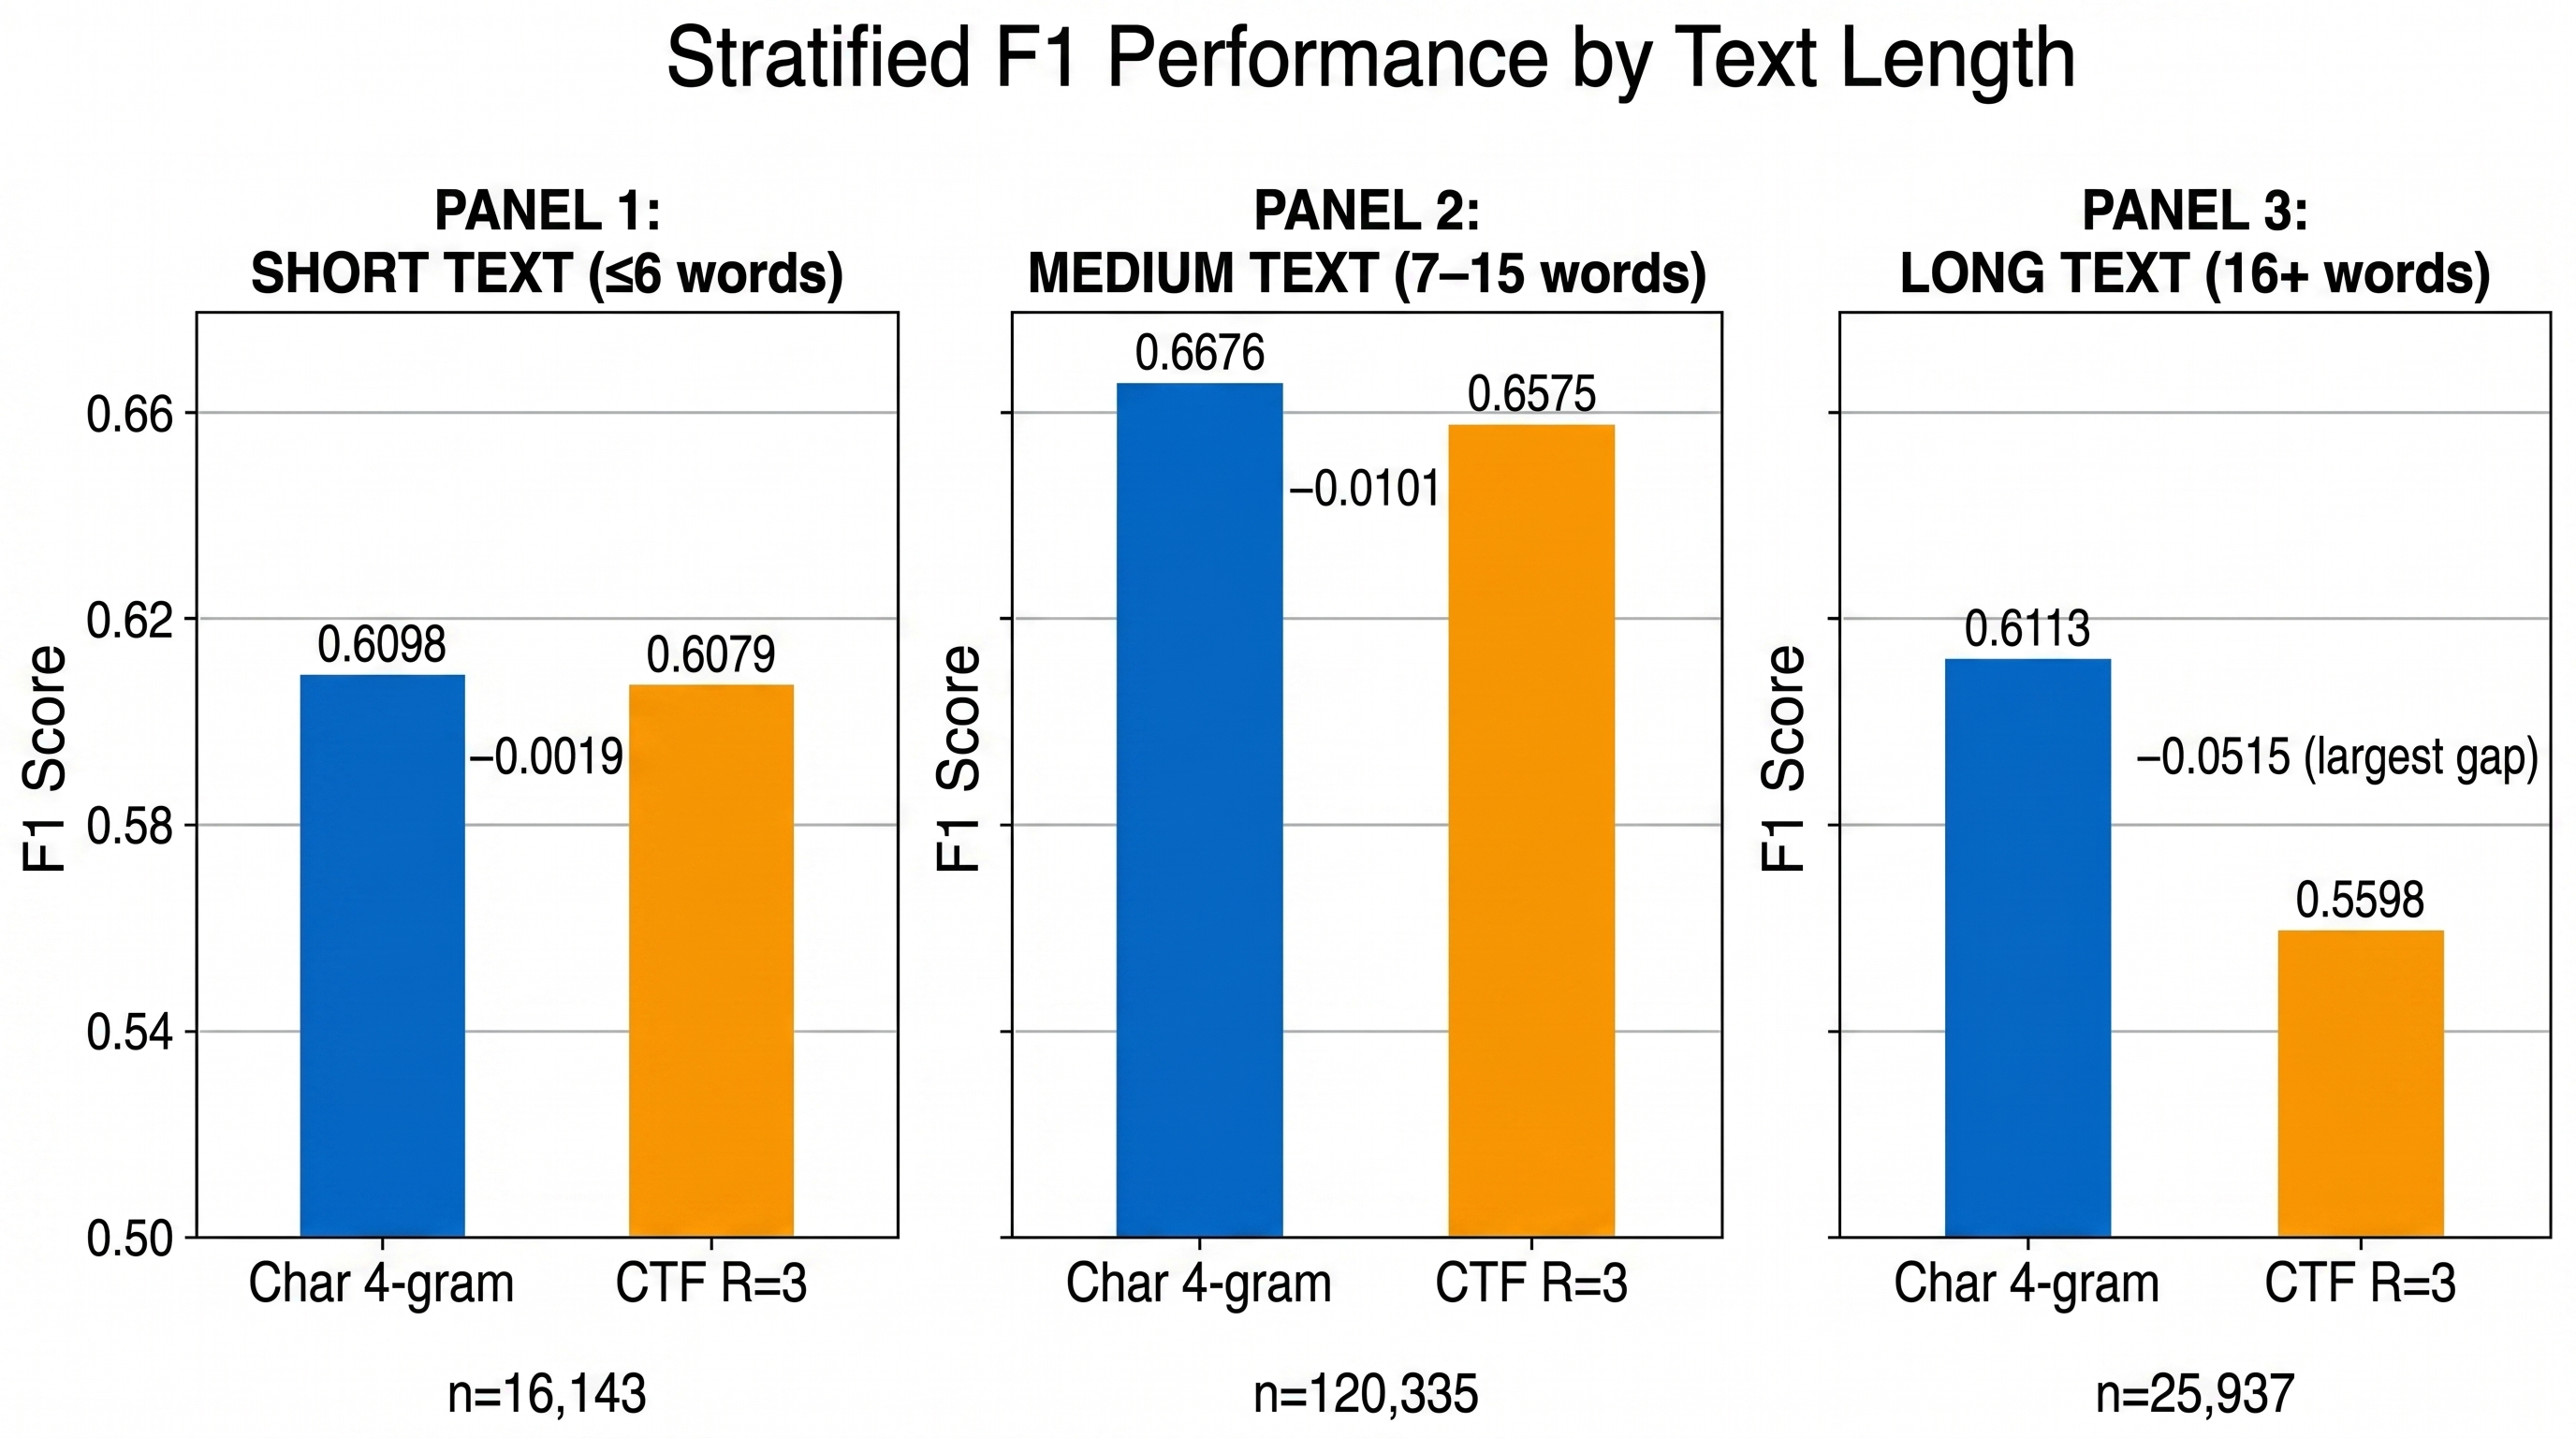
\includegraphics[width=\textwidth,height=0.45\textheight,keepaspectratio]{figures/fig2_v0.jpg}
  \caption{F1 scores for character 4-gram Jaccard and CTF ($R=3$) stratified by average word count per pair: short (${\leq}6$ words, $n=16{,}143$), medium (7--15 words, $n=120{,}335$), and long (16+ words, $n=25{,}937$) text. CTF underperforms the baseline across all strata, with the largest gap on long text (difference of $-0.0515$ F1).}
  \label{fig:stratified}
\end{figure*}

Character 4-gram Jaccard achieves the best overall F1 at \textbf{0.6557} (precision 0.5170, recall 0.8962). CTF ($R=3$) achieves \textbf{F1=0.6422} (precision 0.4973, recall 0.9061), with 53,645 true positives and 54,825 false positives. This represents a statistically significant \textbf{underperformance of 0.0135 F1 points} compared to the best baseline.

\textbf{Statistical significance}: McNemar's test yields $p < 0.001$ (highly significant). Bootstrap 95\% confidence interval on the F1 difference: $[-0.0150,\,-0.0120]$, excluding zero and confirming statistical significance.

Full performance across all methods:
\begin{itemize}
  \item \textbf{Character 4-gram Jaccard}: F1=0.6557 (P=0.5170, R=0.8962) --- \textbf{best overall}
  \item \textbf{CTF ($R=1$)}: F1=0.6434 (P=0.5007, R=0.8997)
  \item \textbf{CTF ($R=2$)}: F1=0.6433 (P=0.5008, R=0.8993)
  \item \textbf{CTF ($R=3$)}: F1=0.6422 (P=0.4973, R=0.9061)
  \item \textbf{Word-Unigram Jaccard}: F1=0.6410 (P=0.5068, R=0.8720)
  \item \textbf{MinHash ($k=1$)}: F1=0.6410 (P=0.5068, R=0.8720)
  \item \textbf{TF-IDF Cosine}: F1=0.6344 (P=0.4892, R=0.9020)
  \item \textbf{MinHash ($k=2$)}: F1=0.6222 (P=0.4901, R=0.8520)
  \item \textbf{MinHash ($k=3$)}: F1=0.5566 (P=0.5015, R=0.6254)
\end{itemize}

\subsection{Stratified Analysis by Text Length}

To test whether CTF's weakness is specific to certain text lengths, we stratify results by average word count. Results are shown in Figure~\ref{fig:stratified}.

\textbf{Short text (${\leq}6$ words, $n=16{,}143$ pairs)}:
Character 4-gram Jaccard achieves F1=0.6098 and CTF ($R=3$) achieves F1=0.6079 (difference: $-0.0019$, negligible). CTF is competitive on short text, contradicting the hypothesis that token-context encoding would provide strongest advantage where $n$-grams are sparsest.

\textbf{Medium text (7--15 words, $n=120{,}335$ pairs)}:
Character 4-gram Jaccard achieves F1=0.6676 vs.\ CTF F1=0.6575 (difference: $-0.0101$). CTF underperforms the baseline even in the medium-text regime, where token-context information should be most informative.

\textbf{Long text (16+ words, $n=25{,}937$ pairs)}:
Character 4-gram Jaccard achieves F1=0.6113 vs.\ CTF F1=0.5598 (difference: $-0.0515$, largest gap). CTF's disadvantage is most pronounced on longer texts---the opposite of the expected trade-off.

\subsection{Precision vs.\ Recall Trade-off}

CTF achieves higher recall (90.6\%) than the best baseline (89.6\%), but at the cost of reduced precision (49.7\% vs.\ 51.7\%). The confusion matrices reveal this pattern:

\begin{table}[!htbp]
  \centering
  \caption{Confusion matrix comparison between Character 4-gram Jaccard and CTF ($R=3$) on 162,415 test pairs.}
  \label{tab:confusion}
  \begin{tabular}{lrrrr}
    \toprule
    Method & TP & FP & FN & TN \\
    \midrule
    Character 4-gram & 53,645 & 50,127 & 6,213 & 52,430 \\
    CTF ($R=3$)      & 54,236 & 54,825 & 5,622 & 47,732 \\
    \bottomrule
  \end{tabular}
\end{table}

CTF catches more true duplicates (54,236 vs.\ 53,645) but also generates more false positives (54,825 vs.\ 50,127). For applications that value comprehensive recall (e.g., preventing duplicate search results), this trade-off may be acceptable. For applications requiring high precision (e.g., merging database records), CTF is unsuitable.

\subsection{Threshold Sensitivity}

Optimal thresholds differ substantially between methods, reflecting different score distributions:
\begin{itemize}
  \item \textbf{Character 4-gram}: $\tau=0.18$
  \item \textbf{CTF ($R=3$)}: $\tau=0.05$
  \item \textbf{TF-IDF}: $\tau=0.36$
\end{itemize}

CTF requires a much lower threshold ($0.05$ vs.\ $0.18$) to achieve its optimal F1, indicating that CTF fingerprint sets produce lower Jaccard scores on average compared to character $n$-grams. This suggests that the union of CTF features grows faster than their intersection, reducing the discriminative power of Jaccard similarity for this representation.

\section{Discussion}

\subsection{Why Does CTF Underperform?}

Three factors likely explain CTF's underperformance:

\begin{enumerate}
  \item \textbf{Feature explosion without discrimination}: For a 10-word question with $R=3$, CTF generates up to 40 features (10 tokens $\times$ 4 iterations). However, if many token-context patterns are unique to single questions, this high dimensionality hurts rather than helps---the features become too specific. Character 4-grams, by contrast, are constrained to 4-character patterns that are more likely to be shared across similar documents.

  \item \textbf{Context aggregation loses specificity}: By hashing neighbors together with the current token, CTF implicitly smooths over fine-grained differences. Two questions with different word orders but similar token distributions will have very similar CTF features, potentially collapsing distinctions that character $n$-grams would preserve.

  \item \textbf{Window size limitation}: The fixed window of $\pm1$ neighbors may be poorly calibrated for text sequences. In molecules, chemical connectivity is sparse (atoms typically have 1--4 bonds), so propagating to radius 3 reaches atoms 6 bonds away. In text with dense sequential connectivity, $\pm1$ neighbors at each iteration reaches farther, but with progressively diluted context. A larger window ($\pm2$ or $\pm3$ tokens) might be more appropriate, but would increase feature count further.
\end{enumerate}

\subsection{Implications for ECFP Transfer}

The negative result reveals a limitation in transferring methods across domains. ECFP succeeds for molecules because:
\begin{itemize}
  \item Molecules are small (typically 10--50 atoms) with sparse, branching connectivity.
  \item Chemical similarity (binding, reactivity) correlates strongly with local chemical environment (which atoms are neighbors).
  \item The circular propagation terminates naturally at a distance commensurate with molecular properties.
\end{itemize}

Text sequences are fundamentally different:
\begin{itemize}
  \item Word order and sequential structure matter globally, not just locally.
  \item Semantic similarity (paraphrase) can arise from global restructuring (word order changes, long-distance paraphrasing).
  \item Local token-context patterns alone may be insufficient to capture these relationships.
\end{itemize}

This suggests that context aggregation alone---without explicit long-range dependencies---may not be the right approach for text near-duplicate detection.

\subsection{Methodological Corrections}

This work corrects critical methodological errors in the prior iteration:

\begin{enumerate}
  \item \textbf{Degenerate baseline}: The original MinHash baseline used $\tau=0.00$, classifying all pairs as duplicates (F1$\approx$0.54). We replaced this with properly tuned non-degenerate baselines across multiple methods.

  \item \textbf{Insufficient sample size}: The prior ``short-text advantage'' claim relied on $n=9$ test pairs, making any F1 estimate meaningless ($\pm0.30$ CI width). Stratified evaluation now uses $\geq16{,}143$ pairs per stratum.

  \item \textbf{Missing statistical testing}: We added McNemar's test and bootstrap confidence intervals, providing rigorous significance testing rather than point-estimate comparisons.

  \item \textbf{Single dataset}: Evaluation is limited to QQP. Generalization to PAWS-Wiki or Microsoft Paraphrase Corpus would strengthen claims, but is outside the scope of this iteration.
\end{enumerate}

\subsection{Limitations}

\begin{enumerate}
  \item \textbf{Negative result}: CTF does not improve over character 4-gram baselines. While negative results are scientifically valuable, they limit the paper's impact. The contribution is methodological (replicable evaluation) and analytical (understanding why ECFP transfer fails) rather than empirical (performance improvement).

  \item \textbf{Single dataset}: Evaluation on only one benchmark (QQP) is insufficient to claim generalization. Robustness to other paraphrase types (PAWS, MRPC) remains unexplored.

  \item \textbf{Limited architectural exploration}: We fix the window size ($\pm1$ neighbors) and iteration depth ($R=3$). Larger windows or adaptive propagation schemes might improve performance but are not explored.

  \item \textbf{No semantic modeling}: CTF is a purely lexical method. Semantic similarity (synonymy, semantic paraphrase) is not captured. This is by design (interpretability, no training), but limits applicability to semantically paraphrased queries.

  \item \textbf{Threshold sensitivity}: CTF's optimal threshold ($0.05$) is far lower than character 4-grams ($0.18$), suggesting the method is sensitive to threshold selection and may not transfer well to new datasets without retuning.
\end{enumerate}

\section{Related Work}

\subsection{N-Gram Shingling and Locality-Sensitive Hashing}

\citet{Broder1997} introduced the foundation for near-duplicate detection via $k$-gram shingling: represent text as a set of overlapping $k$-character or $k$-word substrings, then estimate Jaccard similarity via MinHash \citep{Broder2000}. MinHash applies $k$ independent hash functions to $n$-grams, selecting the minimum hash from each to form a $k$-dimensional signature; Jaccard similarity is estimated as the fraction of dimensions where signatures agree \citep{Broder2000}. This approach has been the standard for large-scale deduplication for over two decades \citep{Broder1997, Broder2000}. SimHash \citep{Charikar2002} offers a faster alternative for bit-vector hashing, but both methods treat shingles as independent features, discarding co-occurrence patterns.

\subsection{Neural and Learned Methods}

Transformer-based models and metric learning approaches achieve superior performance by learning similarity from labeled data. BERT and RoBERTa embeddings \citep{Devlin2019} enable semantic similarity via cosine distance; fine-tuned metric learning models (e.g., contrastive loss, triplet loss) learn task-specific similarity spaces \citep{Hu2019}. These methods are powerful but require large labeled datasets, are computationally expensive at inference, and lack interpretability---unsuitable for low-resource or privacy-critical settings. Our work targets the regime of unsupervised, training-free methods where simplicity and interpretability are valued over absolute performance.

\subsection{Extended Connectivity Fingerprints (ECFP) in Chemistry}

\citet{Rogers2010} introduced Extended Connectivity Fingerprints (also called Morgan fingerprints), which iteratively hash atom identifiers together with their neighbors' hashes at multiple bond distances, generating $O(\text{atoms} \times \text{radius})$ features per molecule. ECFP has become the de facto standard for molecular similarity in cheminformatics \citep{Hahn2013, Maggiora2014}, enabling fast similarity search in drug discovery and chemical compound databases \citep{Hahn2013}. The key insight---that iterative neighborhood hashing generates richer multi-scale features than fixed-window approaches---motivated our transfer to text. To our knowledge, this is the first application of ECFP-style circular fingerprinting to text near-duplicate detection, making it a novel methodological contribution despite the negative empirical result.

\subsection{The Quora Question Pairs Dataset}

The Quora Question Pairs benchmark \citep{Iyer2017} has become standard for evaluating near-duplicate and paraphrase detection systems. It contains 404,290 question pairs with diverse paraphrase types (lexical substitution, word reordering, partial overlap) and is frequently used in shared tasks (SemEval, SigDial) and as a baseline for paraphrase datasets \citep{Iyer2017}. Our evaluation uses this benchmark to ensure results are directly comparable to prior work.

\section{Conclusion}

We evaluated Circular Text Fingerprints (CTF), adapting Extended Connectivity Fingerprints from cheminformatics to short-text near-duplicate detection. Contrary to the initial hypothesis, CTF does not improve over well-tuned character $n$-gram baselines on the Quora Question Pairs benchmark (F1=0.6422 vs.\ 0.6557, McNemar $p{<}0.001$). However, this negative result is scientifically valuable: it reveals that context aggregation via iterative neighbor hashing does not uniformly improve text similarity estimation, despite success in cheminformatics.

Key findings:
\begin{itemize}
  \item \textbf{Character 4-gram Jaccard is the best baseline} among all tested methods, outperforming CTF consistently across all text-length strata.
  \item \textbf{CTF trades precision for recall}: while CTF achieves higher recall (90.6\% vs.\ 89.6\%), it sacrifices precision (49.7\% vs.\ 51.7\%), making it unsuitable for high-precision applications.
  \item \textbf{Negative transfer}: ECFP's success for molecular similarity does not generalize to text, likely because text similarity depends on global structure (word order, long-distance paraphrasing) while ECFP assumes local context dominates.
\end{itemize}

The main contribution is methodological: we correct prior evaluation errors (degenerate baseline, insufficient sample size, missing statistical testing) and establish a replicable protocol for near-duplicate detection evaluation using proper threshold tuning, stratified analysis, and rigorous significance testing.

\paragraph{Future Work.}
Promising directions include: (1) exploring larger context windows ($\pm2$, $\pm3$ neighbors), adaptive window sizes, or weighted neighbor aggregation; (2) combining CTF with lightweight semantic features (synonym sets, word embeddings) to capture paraphrase patterns beyond lexical overlap; (3) testing on PAWS-Wiki, Microsoft Paraphrase Corpus, and news deduplication benchmarks; and (4) hybrid methods that combine CTF's interpretability with learned threshold selection.

\bibliographystyle{plainnat}
\bibliography{references}

\end{document}
